\documentclass[conference]{IEEEtran}
\IEEEoverridecommandlockouts
\usepackage{cite}
\usepackage{amsmath,amssymb,amsfonts}
\usepackage{algorithmic}
\usepackage{graphicx}
\usepackage{textcomp}
\usepackage{xcolor}
\usepackage{lipsum}
\usepackage{blindtext}
\usepackage{subfig}
\usepackage{caption}
\usepackage{placeins}
\usepackage{afterpage}
\usepackage{xurl}
\usepackage{gensymb}
\usepackage{stmaryrd}
\graphicspath{{./images/}}

\definecolor{light-gray}{gray}{0.95}
\newcommand{\size}[2]{{\fontsize{#1}{0}\selectfont#2}}
\newcommand{\code}[1]{\colorbox{light-gray}{\size{8}{\texttt{#1}}}}

\def\BibTeX{{\rm B\kern-.05em{\sc i\kern-.025em b}\kern-.08em
    T\kern-.1667em\lower.7ex\hbox{E}\kern-.125emX}}

\begin{document}

\title{Using Model-Free Deep Reinforcement Learning Algorithms with the MuJoCo Physics Simulator}

\author{
    \IEEEauthorblockN{Curtis Brinker}
    \IEEEauthorblockA{cjbzfd@mst.edu}
    \and
    \IEEEauthorblockN{Tanner May}
    \IEEEauthorblockA{tmay@mst.edu}
}
\maketitle

\begin{abstract}
    \blindtext
\end{abstract}

\section{Introduction}

Recent developments in machine learning have made huge strides in approaching problems that were previously unsolvable with traditional programming methods. In general, machine learning techniques are grouped into three categories:supervised learning, unsupervised learning, and reinforcement learning (RL) \cite{rl_application}. While the first two categories require the whole dataset to train, RL is capable of learning on data as it comes in. This data is formulated as a set of interactions with the agent's environment where each interaction consists of the state of the environment,the action the agent performed, and the resulting state. Thus, agents that use RL learn with a circular process that isa result of the agent's previous actions, known as the agent-environment interaction loop. This complex relationship has given rise to multitudes of algorithms, from remembering a mapping between states and actions to using multiple neural networks to determine the next action.

Like many other areas of machine learning, RL has been revolutionized by the introduction of deep learning. Reinforcement learning algorithms can now learn how to behave in complex, high dimensional environments, such as learning to play videogames with only the pixels as input or how to control a robot. Because of the new found power of RL, we believe that it will play an influential role in the future of AI.

To get experience in this exciting field, we implemented some model-free RL algorithms and taught them how to walk in a 3D environment with the MuJoCo physics simulator.

\section{Testing Environment}

Each of the models were trained using Open AI's Gym library and DeepMind's physics simulator MuJoCo. The Gym toolkit implements numerous environments for testing RL, such as the MuJoCo physics simulator. MuJoCo stands for {\bf Mu}lti-{\bf Jo}int dynamics with {\bf Co}ntact and was made for applications that require fast, accurate physics simulations such as robotics and machine learning \cite{mujoco_docs}. Using MuJoCo, machine learning algorithms can learn how to control the movement of robotic models, such as a snake, ant, or humanoid.

Each of the Gym's environments adhere to a strict structure that makes it easy to switch between environments. One of the most important parts to keep consistent are the values returned after every step of training. Each environment returns the following four values \cite{gym_docs}:

\begin{itemize}
    \item Observation: Represents the current state of the environment, as the agent sees it. In MuJoCo's case, the          environment is fully observable and consists of the model's position, velocity, and various forces \cite{gym_source}
    \item Reward: The reward result of the previous action. The reward for the MuJoCo environment depends on a          number of things and is unique for each model.
    \item Done: A flag denoting if the environment needs to be reset. Each of the models in MuJoCo define a safe height range that the model is allowed to exist within; if the model leaves that range, the done flag is raised and the model is reset back to the start.
    \item Info: Some information useful for debugging.
\end{itemize}

\section{Background}

The study of reinforcement learning is about training an \textit{agent} to interact with an \textit{environment}. An action by an agent can influence the environment, which may later affect the actions of the agent. For this reason, reinforcement learning algorithms must be able handle a changing environment that is causally influenced by the agent itself.

Formalizing the interdependency between the environment and the agent is done with the \textit{agent-environment interaction loop}. In which, at time $t$ the environment is fully described by its \textit{state}, $s_t$. Then, an agent makes an \textit{observation} of the environment, $o_t$, where $o_t \subseteq s_t$.\footnote{While the observation and the state are not necessarily equal, reinforcement learning literature frequently refers to an observation as the state itself.} The agent responds to this observation with an \textit{action} $a_t$ and is given a \textit{reward}, $r_t$. After the action is taken, the state of the environment changes with the new state denoted as $s_{t+1}$.

An environment state can be represented by a tensor of values describing individual aspects of the environment. The domain of possible observations of the agent is referred to as the \textit{observation space}, which can be either continuous or discrete. Similarly, the domain of all actions that an agent can take is called the \textit{action space} which can also be continuous or discrete. An action, $a_t$, is selected from the action space by agent's \textit{policy}. The policy can select actions either deterministically or stochastically. Typically, deterministic policies are denoted with $a_t = \mu(s_t)$ and stochastic policies are denoted as $a_t \sim \pi(\cdot | s_t)$. \cite{spinning_up_intro}



The reward given for the transition from $s_t$ to $s_{t+1}$ by action $a_t$ is given by the reward function, where $r_t = R(s_t, a_t, s_{t+1})$. Though, readers should be aware that some literature refers to this value as $r_{t+1}$. Typically, this reward function is specified by a programmer in a way that rewards a specific goal. With this in mind, the process of training an agent can be formulated as maximizing the cumulative reward, called the \textit{return}. To calculate the return, the \textit{trajectory} is used which contains the sequence of states and actions taken by the agent. The trajectory is given by:
$$
    \tau = (s_0, a_0, s_1, a_1, ...)
$$

Therefore, as the return is defined in terms of cumulative reward, the trajectory can be used to calculate the rewards as the agent interacts with the environment. Then, in its most simple form, the return is the summation of all rewards. However this introduces two problems: First the return for an action $t$ is defined in terms of actions taken before it. Intuitively, we would to only consider rewards that will happen as a result of the current action. Second, The summation of all rewards weights all rewards equally, however, this means that very long term rewards may eventually dominate the summation. To encourage shorter term rewards we can introduce a discount factor, $\gamma$, that discounts the value of future rewards.

Commonly, the reward function $R$ is co-opted to take a trajectory and produce the rewards at each timestep $t$. With these considerations in mind, the return can be defined as:
$$
    R_t(\tau) = \sum_{t'=t}^T \gamma^{t'} r_{t'}, \enspace \gamma \in (0, 1)
$$

Where $T$ is the length of the trajectory and $t$ is the current time for which the return is being calculated. If $T$ is finite, then the return is said to be a \textit{finite-horizon return}. Similarly, if $T$ is infinite, then the return is said to an \textit{infinite-horizon return}. The inclusion of $\gamma$ makes this return a discounted return. This places more focus on near-term rewards and also helps with convergence in infinite-horizon returns. Using $t'$ makes the return only consider future rewards, which \cite{spinning_up_policy_optimization} calls the \textit{reward-to-go} return.

However, an agent cannot act to directly maximize its return as it dependent on future actions and states. Instead, an approximation must be used to calculate the expected return, $\mathcal{J}(\pi)$. This this done with \textit{value functions}. Formally, $\mathcal{J}(\pi)$ is defined as:
$$
    \mathcal{J}(\pi) = \mathop{\mathbb{E}}_{\tau \sim \pi}[R(\tau)]
$$

The \textit{state value function} for policy $\pi$, denoted as $V^\pi$, gives the expected value for policy $\pi$ given state $s$. Alternatively, the \textit{state-action value function} for policy $\pi$, denoted as $Q^\pi$, which can be used estimate the expected value for policy $\pi$ in state $s$ and immediately taking action $a$. Formally, these are defined as:
\begin{align*}
    V^\pi(s)    & = \mathop{\mathbb{E}}_{\tau \sim \pi}[R(\tau) \, | \, s_0 = s]          \\
    Q^\pi(s, a) & = \mathop{\mathbb{E}}_{\tau \sim \pi}[R(\tau) \, | \, s_0 = s, a_0 = a]
\end{align*}

However, these functions are still dependent on the return. To avoid this, we can use the Bellman Equations, which defines both $V^\pi$ and $Q^\pi$ in terms of expected values of future states. \cite{deep_rl_survey, spinning_up_intro, sutton2018reinforcement} These equations are given as:
\begin{align*}
    V^\pi(s_t)      & = \mathop{\mathbb{E}}_{a_t \sim \pi} [ R(s_t, a_t, s_{t+1}) + \gamma V^\pi(s_{t+1})]              \\
    Q^\pi(s_t, a_t) & = \mathop{\mathbb{E}}_{a_{t+1} \sim \pi} [ R(s_t, a_t, s_{t+1}) + \gamma Q^\pi(s_{t+1}, a_{t+1})]
\end{align*}

For the agent to maximize $\mathcal{J}(\pi_\theta)$, the agent must learn to improve the policy $\pi_\theta$, where $\theta$ are the parameters for the policy and is normally updated by gradient ascent. Normally this involves using $V^\pi$ or $Q^\pi$ to better approximate the optimal value functions. Commonly, these approximation are done via deep neural networks. The exact details of how the policy and value function(s) are updated is dependent on the reinforcement learning algorithm used. Following is a brief discussion on different types of reinforcement learning algorithms followed by discussions on details of specific algorithms studied in this paper.

A simplified taxonomy of deep reinforcement learning algorithms is given by \cite{spinning_up_taxonomy}. At the highest level, reinforcement learning algorithms can be split into two categories, \textit{model-based} or \textit{model-free}. Model-based algorithms learn the state transition function, allowing it to predict future states of the environment. Learning the world model has many benefits that can drastically increase the performance of an agent, however, doing so significantly increases the complexity of the algorithms and is outside the scope of this paper. Model-free algorithms do not learn to predict the environment and instead learn other functions to increase the agent's return. Model-free algorithms can be further categorized as using \textit{policy optimization} or \textit{Q-learning}.\footnote{Policy optimization and Q-learning are not mutually exclusive categories.}

Policy optimization algorithms train by optimizing the parameters of the policy $\pi_\theta$. This is normally done learning a value approximator $V_\phi$ and sampling actions taken by the current policy to update parameters accordingly. Because this process requires actions from the current policy, these techniques are considered to be \textit{on-policy}.

Another approach, though not necessarily mutually exclusive, is using Q learning. These algorithms learn an approximator $Q_\theta$ to determine the value of state action pairs. An advantage to this technique is that it can learn from past experiences that were not from the current policy. Algorithms that can learn from experiences of different policies are called \textit{off-policy}. Actions by these algorithms typically are chosen by selecting the action that maximizes $Q_\theta(s, a)$ for the current state $s$.

\subsection{The REINFORCE Algorithm}

One of the simplest forms of policy optimization algorithms is a class of algorithms presented by Williams as REINFORCE. \cite{REINFORCE} The core idea this algorithm is to update the policy by sampling trajectories from the policy. Once a sample has been taken from the current policy, the policy $\pi_\theta$ and value approximator $V_\phi$ can be updated. There is some flexibility in how the parameters are updated, though \cite{spinning_up_policy_optimization} provides some examples of frequently used techniques. The policy is updated using gradient ascent where the gradient is given by:
$$
    \nabla_\theta\mathcal{J(\pi_\theta)} = \mathop{\mathbb{E}}_{\tau \sim \pi_\theta} \left[\sum_{t=0}^{T}\nabla_\theta \, log \, \pi_\theta(a_t | s_t) \, \Phi_t \right]
$$
\begin{flushleft}
    Where $\Phi_t$ is any function that is independent of $\theta$.
\end{flushleft}


To update the value approximator parameters $\phi$, it is common to use gradient descent on a loss such as mean squared error on the value approximator and the reward-to-go return.
$$
    \mathcal{L}(\phi) = \mathop{\mathbb{E}}_{\tau \sim \pi_\theta} \left[\left(V_\phi(s_t) - R_t(\tau)\right)^2\right]
$$

\subsection{Advantage Actor Critic (A2C)}

The advantage actor critic is an on-policy algorithm based on the REINFORCE algorithm. A2C was first proposed by \cite{A2C} along with an asynchronous variant called A3C. The details about the asynchronous version of the algorithm is not pertinent to this paper and will not be discussed. As a whole, there are two main techniques used to improve the performance of this algorithm.

The first technique is the use of the advantage function, $A^{\pi_\theta}(s_t, a_t)$ as $\Phi_t$. The advantage function is defined as:
$$
    A^{\pi_\theta}(s_t, a_t) = Q^{\pi_\theta}(s_t, a_t) - V^{\pi_\theta}(s_t, a_t)
$$

It should be noted that $\Phi_t$ must be independent of $\theta$ and by consequence $a_t$. However, \cite{spinning_up_policy_optimization} provides a proof that $A^{\pi_\theta}(s_t, a_t)$ can be written it terms of $s_t$ only. The advantage can be thought of as quantifying how much better an action in a given state is than average. Negative values signify that the action was less than expected value for the given state, and positive signifies that it was better. Mathematically, the advantage function useful as subtracting by $V^{\pi_\theta}(s_t)$ reduces the variance in the policy gradient leading to more stable learning.

The second technique is the use of an actor-critic framework. The idea of this framework it to separate the concerns of learning different aspects of training. The actor is tasked with learning the policy that will interact with the environment. The critic is tasked with learning the value function that it will use to criticize the actor's actions. \cite{deepmind_slides_9}

\subsection{Deep Deterministic Policy Gradient (DDPG)}

DDPG is an off-policy learning algorithm for continuous action spaces that was proposed by \cite{DDPG}. It learns a Q function and a deterministic policy to select actions and uses a variety of techniques to improve performance and stability of the algorithm. An overview of unique methods used by this algorithm is provided by \cite{spinning_up_ddpg}. One technique that is commonly used by off-policy algorithms is the use a replay buffer. Because off-policy algorithms can learn from actions that did not originate from the current policy, past experiences can be stored in a buffer. Then, during training, a larger sample size can be used to improve training.

To update the function $Q_\phi$, gradient descent is used on $\phi$ to minimize the mean squared error of $Q_\phi(s, a)$ and the \textit{target}, where the target is defined as:
$$
    y = r + \gamma(1-d)Q_\phi(s', \mu_\theta(s'))
$$

Where $(s, a, r, s', d)$ is a transition in the replay buffer $\mathcal{D}$. The resulting state from the action is $s'$ and $d$ is the \textit{done} flag where $d=1$ if $s'$ is a terminal state, $d=0$ otherwise. Additionally, $\mu_\theta$ is the deterministic policy used to select the next action.

However, using gradient descent the mean squared error of $Q_\phi$ and $y$ is problematic as $y$ is also dependent on $\phi$. As a result, both $Q_\phi$ and $y$ change when $\phi$ is updated, leading to instability. To resolve this, DDPG uses \textit{target networks}, which uses polyak averaging to remove this direct dependency. The target networks, $Q_{\phi'}$ and $\mu_{\theta'}$ have the same structure as their original networks but are updated as follows:
\begin{align*}
    \phi'   & \leftarrow \rho \, \phi' + (1 - \rho) \phi     \\
    \theta' & \leftarrow \rho \, \theta' + (1 - \rho) \theta
\end{align*}

This provides stability to the loss function, therefore $Q_\phi$ is updated using gradient descent on
$$
    \mathcal{L}(\phi, \mathcal{D}) = \mathop{\mathbb{E}}_{(s,a,r,s',d) \sim \mathcal{D}}\left[\left(Q_\phi(s,a) - y\right)^2\right]
$$
\begin{flushleft}
    Where $y$ is the target, which is calculated as:
\end{flushleft}
$$
    y = r + \gamma(1-d)Q_{\phi'}(s', \mu_{\theta'}(s'))
$$

To update the policy, we want to maximize the value function $Q_\phi$ using $\mu_\theta$. To do this, the following loss function is used:
$$
    \mathcal{L}(\theta, \mathcal{D}) = \mathop{\mathbb{E}}_{s \sim \mathcal{D}}\left[-Q_\phi(s, \mu_\theta(s))\right]
$$

Finally, to gain additional benefit from the algorithm off-policy, DDPG uses another technique to encourage exploration during train time. This is done by adding random noise to actions to stray away from the deterministic policy. The original authors uses OU noise, however \cite{spinning_up_ddpg} recommends a zero centered Gaussian distribution which is simpler to implement and still effective.

\subsection{Soft Actor Critic (SAC)}

\blindtext

\section{Methodology}

Each of the algorithms were implemented on Ubuntu 20.04 with Python 3.8 using the PyTorch library. We used PyTorch because we had previous experience with it and liked how flexible it is compared to other options. To train the models, we used the previously mentioned Gym library. To verify that the implementation of each of the algorithms worked correctly, they were trained in the CartPole and Pendulum environments. For training towards the goal, the Ant-v3 and Humanoid-v3 MuJoCo models were used.

The hyperparameters for each algorithm were as follows:
\begin{itemize}
    \item A2C: Learning rate of $3e^{-4}$ and $\gamma = 0.99$.
    \item DDPG: Update freq. of 64 steps, update threshold of 4096 steps, batch size of 128, learning rate of $1e^{-3}$, $\gamma = 0.99$, $\tau = 0.995$, and the noise distribution was Gaussian with a standard deviation of 0.1 (\cite{DDPG} used OU noise, but \cite{spinning_up_ddpg} recommended using the easier to implement Gaussian noise).
    \item SAC: Update freq. of 64 steps, 64 updates per update step, an update threshold of 4096 steps, batch size of 128, $\alpha = 0.5$, learning rate of $5e^{-4}$, $\gamma = 0.99$, $\tau = 0.995$, and an $\alpha$ decay of 1.
\end{itemize}
Each of those parameters were chosen because they resulted in the best performing model.

Since the goal is to teach Deep RL algorithms how to walk, the networks for each of the algorithms were defined to have two layers, each with 256 neurons. Originally the layers had 128 neurons each but tests using the 256 neuron configuration resulted in better performance. More layers and neurons can, of course, be used but would have greatly increased the computational cost of training.

Since every environment has its own quirks, each is described in its own subsection below \cite {gym_source}.

\subsection{CartPole-v0}

The objective of the CartPole environment is to teach an agent to balance a pole on a cart by moving the cart left and right. The environment has a continuous observation space consisting of the cart's position, the cart's velocity, the pole's angle, and the pole's angular velocity. The action space is discrete with the options of moving the cart to the left or to the right. The environment rewards the agent with a value of one, simply for staying healthy.

Initially, the values of both the cart and pole are randomly sampled from a uniform distribution from $[-0.5, 0.5]$. The environment is terminated when the angle of the pole is $\pm12\degree$, the cart position hits the edge of the display,or when the length of the episode surpasses 200 steps. The environment is considered solved when the reward is\textgreater 195 for 100 consecutive episodes.

This environment was used as a proof of concept of each algorithm's implementation.

\subsection{Pendulum-v1}

The pendulum environment's objective is to balance a frictionless pendulum straight up. The observation space is continuous and describes the angle of the pendulum as well as the angular velocity. The action space is also continuous and details the amount of left or right force to apply to the pendulum. The reward incentivizes keeping the pole at an angle of $0\degree$ with as little velocity and force as possible. The reward is formulated as
$$
    R = -(angle ^{2} + 0.1 * angular\_velocity ^ {2} + 0.001 * action ^ {2})
$$
Since the angle is normalized between $[-\pi, \pi]$ before calculating the reward, the reward has a range of$[-16.3, 0]$.

The environment's initial state has the pole at a random angle between $[-\pi, \pi]$ radians with a random velocity between $[-1, 1]$. The environment does not specify a termination state, so a limit of 150 was imposed. Similarly, the environment does not specify when it is solved, so it was allowed to run until it hit the step limit.

Like the CartPole environment, this environment was used as another proof of concept of the implementation for each algorithm.

\subsection{Ant-v3}

The ant is a sphere with four legs, each with two joints. The continuous observation space is significantly more complex than the previous environments: it consists of the model's position, velocity, and the forces between the legs and the ground (contact force). The action space is also continuous and describes where and how quickly to move each joint. The reward encourages the model to move as quickly as possible while moving as few joints as little and softly as possible. It is formulated as
$$
    R = (v + h) - (a + f)
$$
where $v$ is the velocity in the x-axis, $h$ is the healthy reward configured to be 1, $a$ is the control\_cost calculated by $0.5* \sum actions^{2}$, and $f$ is the contact\_cost calculated by $5e^{-4} * \sum contact\_forces^{2}$.

The environment starts with each joint in a random position with a random velocity. The episode is terminated when the model exits the safe height range of $[0.3, 2.0]$. The environment did not define a solve condition so the episode was continued until the model made a mistake to trigger the termination condition.

The ant was chosen because it is the simplest provided model that meets the "three dimensional walker" condition. Each of the algorithms had 500,000 episodes to train using this model. After training was stopped, the most recently saved model was used for analysis. A training length of 500,000 episodes was used because it consistently produced an agent that could walk a non-trivial distance.

\subsection{Humanoid-v3}

The humanoid model is a humanoid with two legs, two arms, a head and a torso. The legs, arms, and torso are made up of multiple joints, each individually controlled. Like the ant, the observation space is continuous and describes the model's position, the model's velocity, the forces for each of the joints, and the contact forces. The environment also defines a continuous action space that describes the new position and velocity of each joint. The intuition for the reward is the same as for the Ant environment, but it is calculated slightly differently where $v$ is equal to $1.25 * x\_velocity$, $h$ is configured to be 5, $a$ is calculated as $0.1 * \sum actions^{2}$, and $f$ is defined as $5e^{-7} * \sum contact\_forces^{2}$.

Like the Ant environment, the model starts with each joint in a random position and random velocity. The episode is terminated when the model exits the safe height range of $[1.0, 2.0]$. The environment did not define a solve condition so the episode was continued until the model made a mistake to trigger the termination condition.

The humanoid was chosen because it is the most complex 3D walker and showcased the learning power of the tested algorithms. Since this model is significantly more complex than the Ant, 1,250,000 episodes were used for training. But due to the cost of training, only SAC was trained with this model.

\section{Results}

<Why does loss not matter; only need to see that the reward is trending upward>
<in the following sections be sure to mention why SAC is impressive>

\blindtext

\subsection{CartPole-v0}

\blindtext

\subsection{Pendulum-v1}

\begin{figure}
    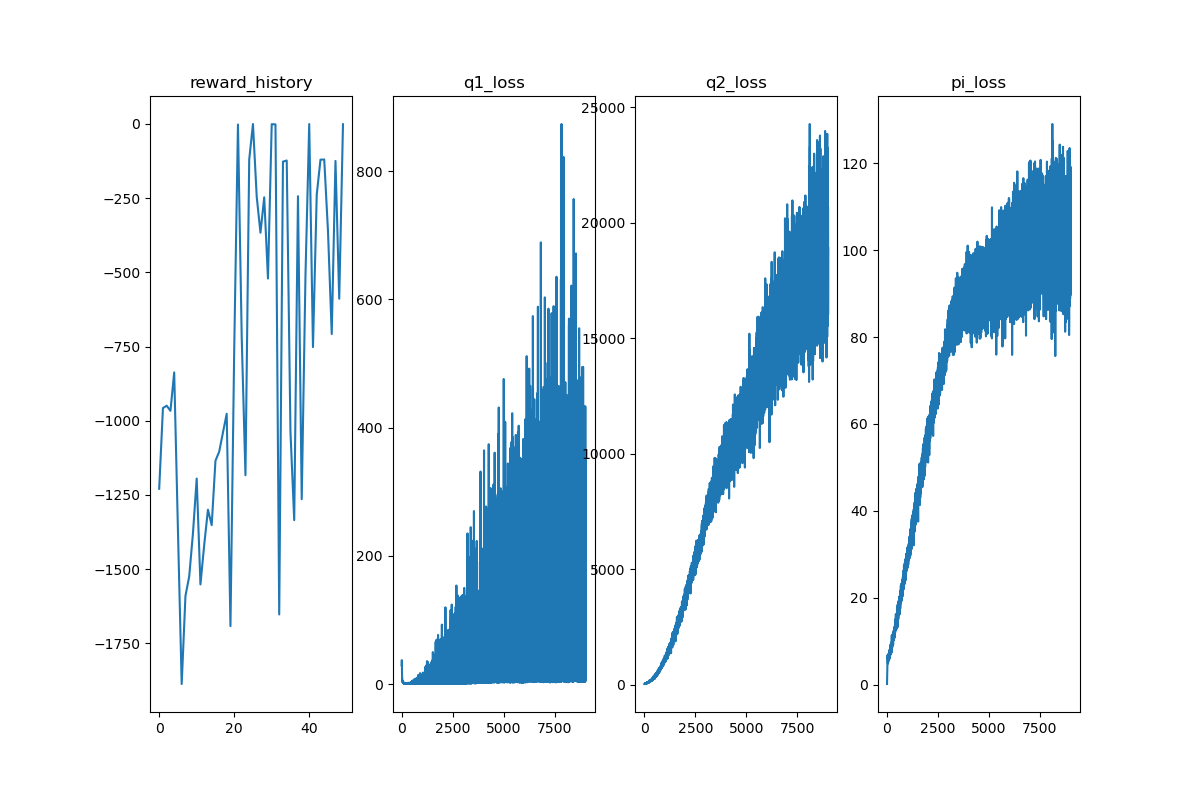
\includegraphics[width=0.45\textwidth]{sac-pendulum}
    \caption{SAC in the Pendulum-v1 Environment}
\end{figure}

\blindtext

\subsection{Ant-v3}

<SAC jumped, DDPG walked>
<SAC reward increase is steeper than DDPG's>
<mention SAC jumping/leaping>

\begin{figure}
    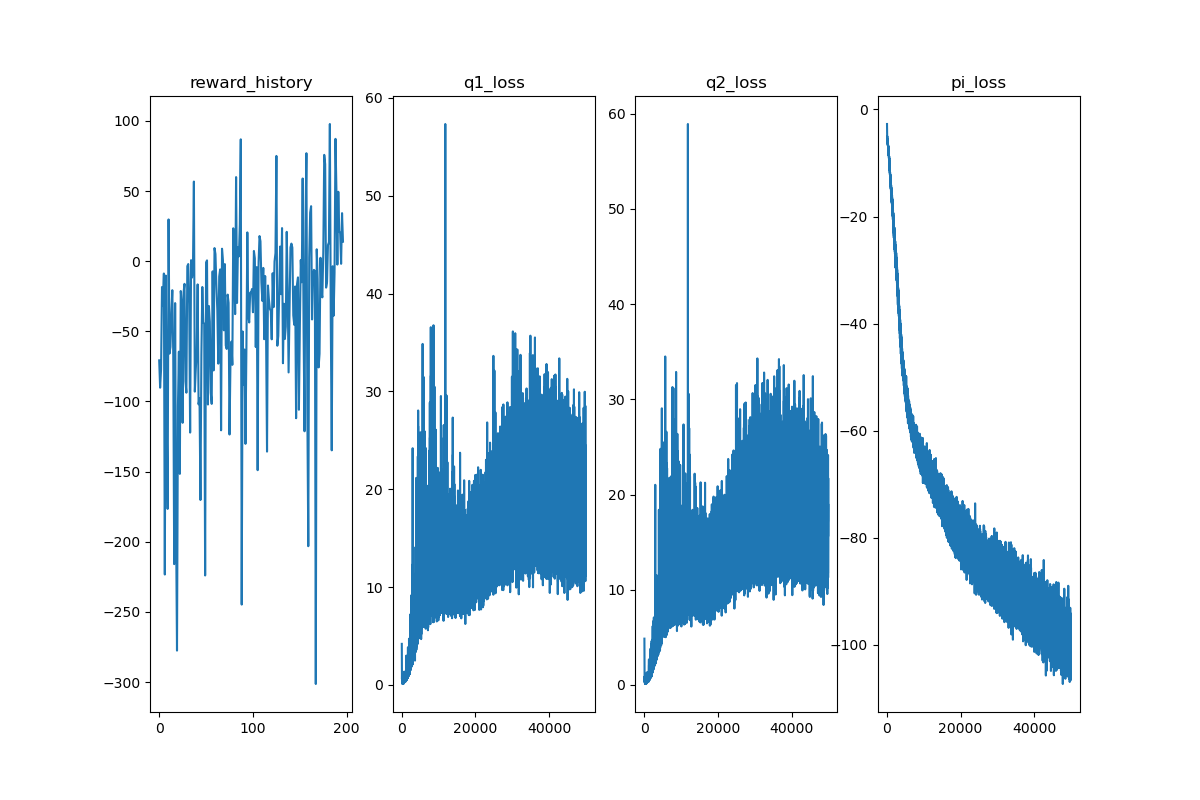
\includegraphics[width=0.45\textwidth, height=5cm]{sac-ant}
    \caption{SAC in the Ant-v3 environment}
\end{figure}

\begin{figure}
    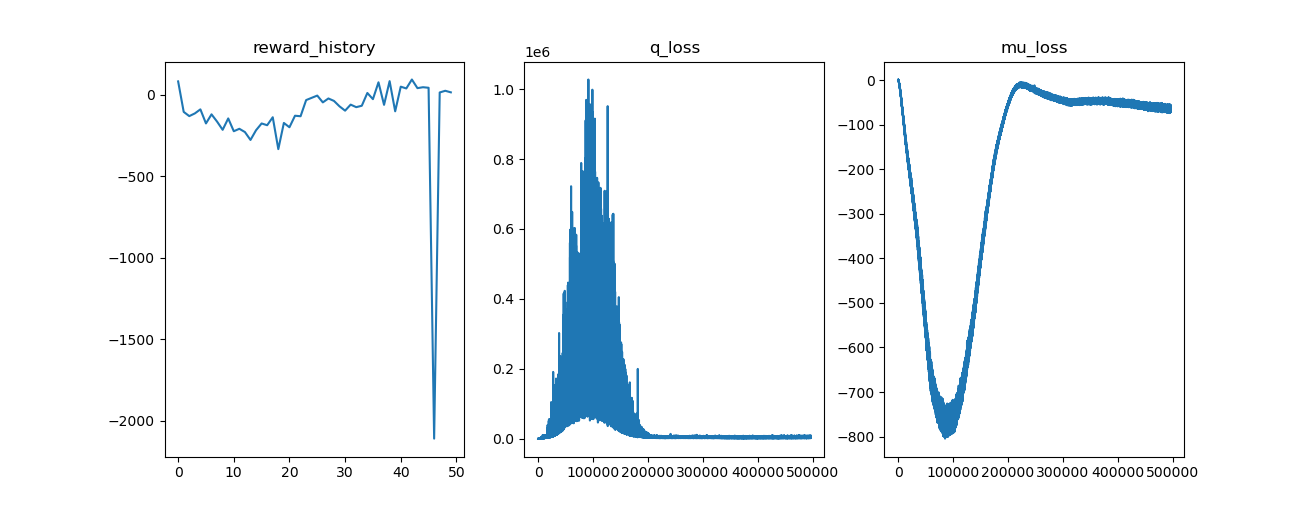
\includegraphics[width=0.45\textwidth, height=5cm]{ddpg-ant}
    \caption{DDPG in the Ant-v3 environment}
\end{figure}

\blindtext

\subsection{Humanoid-v3}

<model shuffled along instead of taking steps>

\begin{figure}
    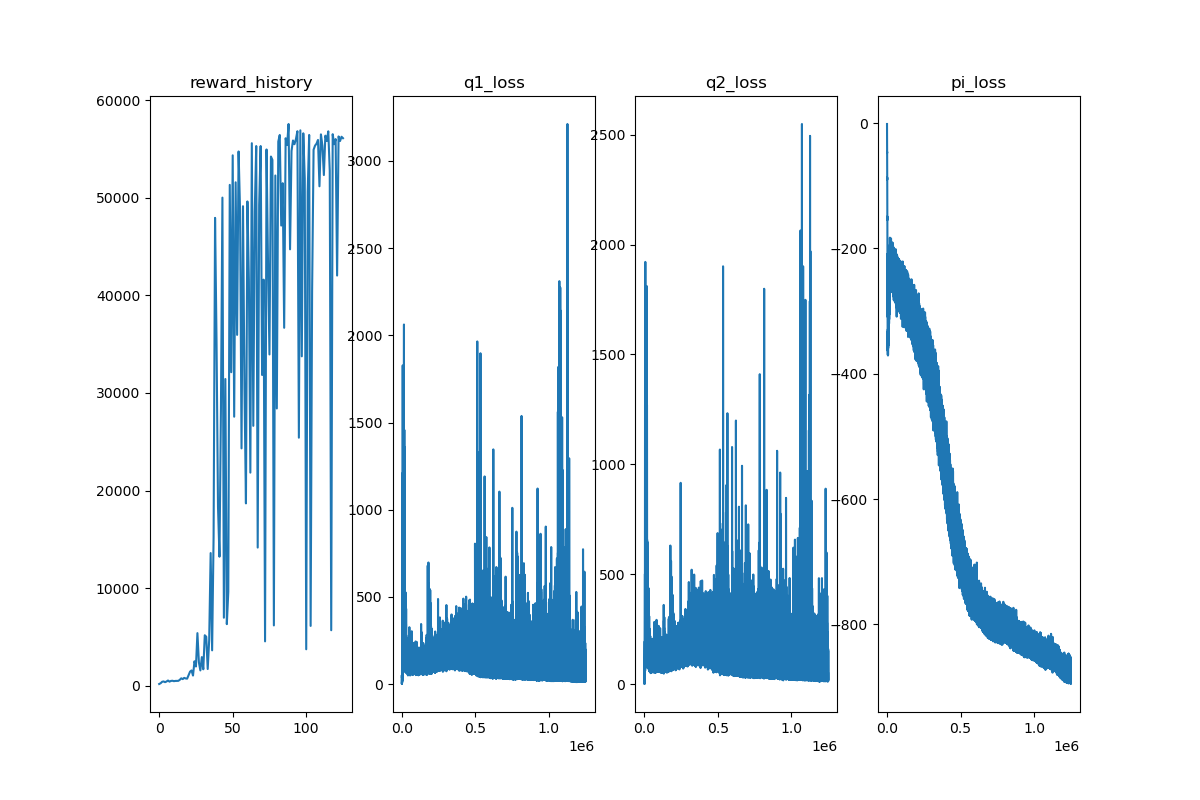
\includegraphics[width=0.45\textwidth, height=5cm]{sac-humanoid}
    \caption{SAC in the Humanoid-v3 environment}
\end{figure}

\blindtext

\section{Conclusions and Future Work}

Learning to walk is a challenging problem; multiple limbs have to move in a coordinated fashion just to keep balance, adding movement on top of that is a problem that is potentially unsolvable with conventional programming methods. Using Reinforcement learning algorithms, the agent learned, not only, to move a complex model in a 3D environment, but in the case of Soft Actor Critic, to leap its way to success. By implementing and training these algorithms, we are also leaping into success: we now have a solid foundation to begin building new experiences in Reinforcement Learning. We learned the basics of RL like the value and policy functions, policy gradients, and a dictionary's worth of RL vocabulary, all of which will propel us into the future of RL in research and industry.
To continue learning about RL with MuJoCo, we can implement more algorithms or train with different kinds of models, a bicycle perhaps? But reinforcement learning has a much broader scope than just MuJoCo, we could move on to Multiagent learning for games like Chess \cite{multiagent}, learning how to play complex single play video games like Dark Souls, or even self driving \cite{self_driving}. Our new foundational knowledge of RL leaves us well equipped to keep up with research and potentially contribute some day our selves.

\bibliography{references}
\bibliographystyle{ieeetran}


\end{document}
